\begin{activity}{Building a Geotherm}

\section*{Purpose}
Every steady-state geotherm you have interpreted so far in this workshop -- the refraction problem, the layered/anisotropic conductivity problem, the velocity-based heat production estimate -- has depended on a geotherm existing without ever building one from scratch. This activity does that: given $k(z)$, $A(z)$, a surface temperature $T_0$, and a surface heat flow $q_0$, you will construct a full steady-state geotherm by hand, in two separate stages, and follow it all the way to the mantle adiabat.

\section*{Learning Outcomes}
By the end of this activity, you should be able to:
\begin{itemize}
  \item List the ingredients needed to compute a steady-state geotherm, and identify which equation needs which of them.
  \item Compute $q(z)$ and $T(z)$ using a two-stage piecewise method, and explain why $q(z)$ can be completed before $T(z)$ is ever touched.
  \item Interpret the depth at which a conductive geotherm meets the mantle adiabat as the base of the thermal lithosphere.
  \item Predict and explain how changes in $k$ and in $A$ reshape a geotherm differently -- including a case where \emph{more} heat production produces \emph{lower} temperatures.
\end{itemize}

\section*{Geological Context}
\begin{figure}[h]
  \centering
  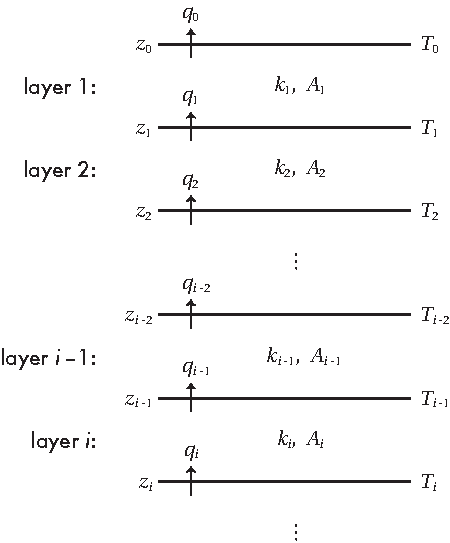
\includegraphics[]{figures/thermal_layers}
  \caption{Layered Earth model for 1-D geotherms assuming constant physical property layers (or sublayers).}
  \label{fig:layers}
\end{figure}
Assuming a layered Earth within which the properties thermal conductivity and heat production are constant (Figure~\ref{fig:layres}), we can write the above expressions as
\[
  q_{i} = q_i-1 - A_{i} (z_{i} - z_{i-1}) \quad \text{where $x \in [1\ldots N]$} ,
  \label{eq:heat_flow}
\]
and
\[
  T_{i} = T_{i-1} 
  + \frac{q_{i-1}}{k_i} (z_i - z_{i-1}) 
  - \frac{A_i}{2 k_i} (z_i - z_{i-1})^2 \, ,
  \label{eq:temperature}
\]
where $i$ denotes the layer and $N$ the total number of layers.  We can further simplify the calculations by defining $\Delta z_i = z_i - z_{i-1}$.  Note that temperature and heat flow are determined at the top and bottom of and the physical properties are defined within each layer.

Notice that the first equation involves only $A(z)$ and $q_0$ -- not $k$ or $T$. The second equation needs $q(z)$, which means it cannot be started until the first is finished. That ordering is not a computational convenience; it is a real physical fact about which quantities depend on which.

Eventually, a conductive geotherm should meet the \textbf{mantle adiabat}, which can be approximated as $T = 1300 + 0.3 z$ ($z$ in km, $T$ in $^\circ$C). The adiabatic temperature profile is the temperature path mantle material follows during convection, which controls how heat moves. The depth these two temperature paths cross marks the base of the thermal lithosphere.

\section*{Tasks}
\begin{questions}

  \question{The Recipe}

  \begin{enumerate}[label=(\alph*)]
    \item From the two equations above, list everything you need to know before you can compute a geotherm.
    \answerbox[2cm]

    \item Which of those quantities does $q(z)$ actually depend on? Which does $T(z)$ depend on that $q(z)$ does not?
    \answerbox[2cm]
  \end{enumerate}

  \question{Stage 1: Building $q(z)$}
  Our crustal column has the layers below, with surface boundary conditions: $q_0 = \SI{60}{mW.m^{-2}}$ and $T_0 = \SI{15}{\circ C}$. 

  \begin{center}
    \begin{tabular}{lccc}
      \toprule
      Layer & Depth range & $k_i$ & $A_i$ \\
      & \si{km} & \si{W.m^{-1}.K^{-1}} & \si{\mu W.m^{-3}} \\
      \midrule
      upper crust  & 0--15  & 3.0 & 1.5 \\
      lower crust  & 15--40 & 2.1 & 0.2 \\
      upper mantle & 40+    & 3.5 & 0.02 \\
      \bottomrule
    \end{tabular}
  \end{center}

  Complete the table below. At each step, using equation~\ref{eq:heat_flow} and $A_i$ of whichever layer that step falls in. The first step is worked for you.

  \begin{center}
    \begin{tblr}{
      colspec = {clcX[c]X[c]},
      row{5-9} = {ht=2.5em},
      hline{1,3,10} = {solid},
      hline{4-9} = {dashed},
      vline{1,4,6} = {solid},
      vline{5} = {dashed}
    }
      $z_i$ & Layer & $\Delta z_i$ & $A\cdot\Delta z_i$ & $q_i$ \\
      \si{km} & & \si{km} & \si{mW.m^{-2}} & \si{mW.m^{-2}} \\
      0   & --           & --  & --   & 60.0 \\
      5   & upper crust  & 5   & 7.5  & 52.5 \\
      10  & upper crust  & 5   &      & \\
      15  & upper crust  & 5   &      & \\
      40  & lower crust  & 25  &      & \\
      80  & upper mantle & 20  &      & \\
      100 & upper mantle & 20  &      & \\
    \end{tblr}
  \end{center}

  \question{Stage 2: Building $T(z)$}
  Now use your completed $q(z)$ column to estimate temperatures using Equation~\ref{eq:temperature}.  The first step is worked for you.

  \begin{center}
    \begin{tblr}{
      colspec = {ccccX[c]X[c]},
      row{5-9} = {ht=2.5em},
      hline{1,3,10} = {solid},
      vline{4-9} = {dashed},
      vline{1,5,7} = {solid},
      vline{2,3,6} = {dashed}
    }
      $z_i$ & $\Delta z_i$ & $k_i$ & $A_i$ & $q_i$ & $T_i$ \\
      \si{km} & \si{km} & \si{W.m^{-1}.K^{-1}} & \si{K} & \si{mW.m^{-2}} & \si{^\circ C} \\
      0   & --  & --  & --   & 60.0 & 15.0 \\
      5   & 5   & 3.0 & 1.5  & 52.5 & 108.75 \\
      10  & 5   & 3.0 & 1.5  &      & \\
      15  & 5   & 3.0 & 1.5  &      & \\
      40  & 25  & 2.1 & 0.2  &      & \\
      80  & 20  & 2.1 & 0.02 &      & \\
      100 & 20  & 2.1 & 0.02 &      & \\
    \end{tblr}
  \end{center}

  Your temperature result at \SI{40}{km} depth is the Moho temperature.

  \question{Plotting the Geotherm}
  Plot your Stage 1 \& 2 results along with the table below which fills in some of the gaps.  Draw a curve through the dots. Also plot the mantle adiabat $T = 1300 + 0.3 z$ (two points are enough since it's a straight line). A more realistic adiabat is slightly more complex, but not by much.

  \begin{center}
    \begin{tabular}{clcc}
      \toprule
      $z_i$ & Layer & $q(z_i)$ & $T(z_i)$ \\
      \si{km} & & \si{mW.m^{-2}} & \si{^\circ C} \\
      \midrule
      20  & lower crust         & 36.5 & 347 \\
      25  & lower crust         & 35.5 & 433 \\
      30  & lower crust         & 34.5 & 516 \\
      35  & lower crust         & 33.5 & 597 \\
      50  & mantle lithosphere  & 32.3 & 768 \\
      60  & mantle lithosphere  & 32.1 & 860 \\
      70  & mantle lithosphere  & 31.9 & 951 \\
      90  & mantle lithosphere  & 31.5 & 1133 \\
      100 & mantle lithosphere  & 31.3 & 1222 \\
      110 & mantle lithosphere  & 31.1 & 1311 \\
      \bottomrule
    \end{tabular}
  \end{center}

  \begin{figure}[h]
      \centering
      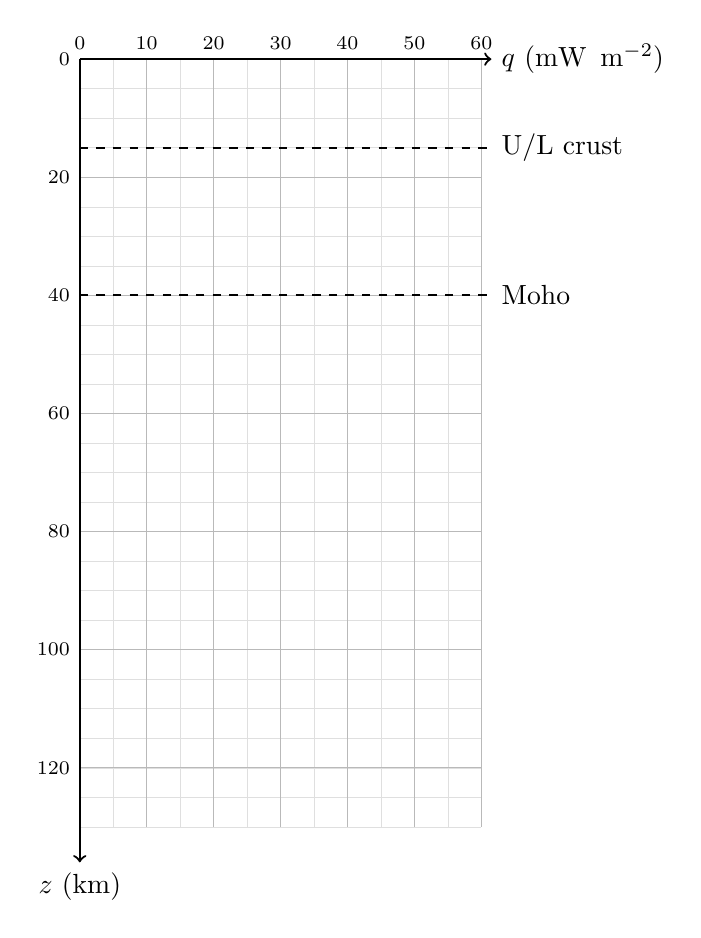
\begin{tikzpicture}[x=0.85cm, y=-0.75cm]
        \draw[gray!25, very thin, xstep=0.5, ystep=-0.5] (0,13) grid (6,0);
        \draw[gray!55, thin, xstep=1, ystep=-2] (0,13) grid (6,0);
        \draw[thick,->] (0,0) -- (6.15,0) node[right] {$q$ (mW\, m$^{-2}$)};
        \draw[thick,dashed] (0,1.5) -- (6.15,1.5) node[right] {U/L crust};
        \draw[thick,dashed] (0,4) -- (6.15,4) node[right] {Moho};
        \draw[thick,->] (0,0) -- (0,13.6) node[below] {$z$ (km)};
        \foreach \q/\qlab in {0/0,1/10,2/20,3/30,4/40,5/50,6/60}
          \node[above, font=\scriptsize] at (\q,0) {\qlab};
        \foreach \zz/\zlab in {0/0,2/20,4/40,6/60,8/80,10/100,12/120}
          \node[left, font=\scriptsize] at (0,\zz) {\zlab};
      \end{tikzpicture}
      \hfill
      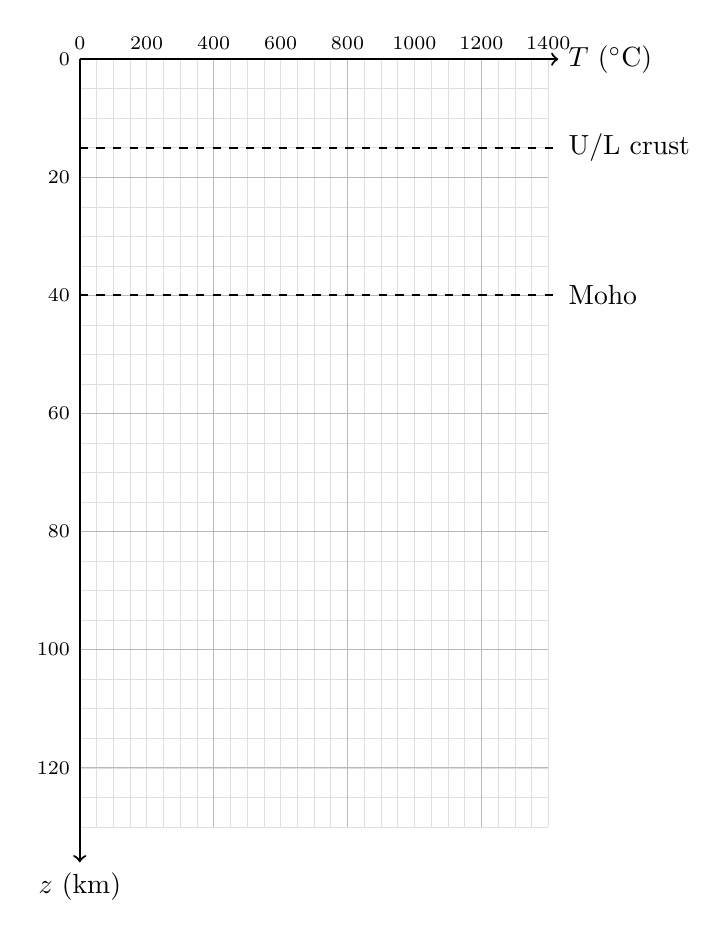
\begin{tikzpicture}[x=0.85cm, y=-0.75cm]
        \draw[gray!25, very thin, xstep=0.25, ystep=-0.5] (0,13) grid (7,0);
        \draw[gray!55, thin, xstep=2, ystep=-2] (0,13) grid (7,0);
        \draw[thick,->] (0,0) -- (7.15,0) node[right] {$T$ ($^\circ$C)};
        \draw[thick,dashed] (0,1.5) -- (7.15,1.5) node[right] {U/L crust};
        \draw[thick,dashed] (0,4) -- (7.15,4) node[right] {Moho};
        \draw[thick,->] (0,0) -- (0,13.6) node[below] {$z$ (km)};
        \foreach \t/\tlab in {0/0,1/200,2/400,3/600,4/800,5/1000,6/1200,7/1400}
          \node[above, font=\scriptsize] at (\t,0) {\tlab};
        \foreach \zz/\zlab in {0/0,2/20,4/40,6/60,8/80,10/100,12/120}
          \node[left, font=\scriptsize] at (0,\zz) {\zlab};
      \end{tikzpicture}
    \caption{Axes for plotting heat flow and geotherms.}
    \label{fig:gtherm-ax}
  \end{figure}

  \begin{enumerate}[label=(\alph*)]
    \item How does heat flow change between the crustal layers when heat production is constant within the layer?
    \answerbox[2cm]

    \item Where is the temperature curvature most visible on your plot -- and where is the curve closest to a straight line? Does that match which layers have the largest $A$?
    \answerbox[2.5cm]

    \item What does the depth where your geotherm meets the adiabat physically represent?
    \answerbox[2cm]
  \end{enumerate}

  \question{Changing $k$}
  Recompute \emph{only} $T(z)$ (not $q(z)$ as $A(z)$ has not changed) using $k_1'=\SI{1.5}{W.m^{-1}.K^{-1}}$ for the upper crust instead of 3.0.  Plot the result on the same axes above.

  \begin{center}
    \begin{tblr}{
      colspec = {ccccX[c]X[c]},
      row{5-9} = {ht=2.5em},
      hline{1,3,10} = {solid},
      vline{4-9} = {dashed},
      vline{1,5,7} = {solid},
      vline{2,3,6} = {dashed}
    }
      $z_i$ & $\Delta z_i$ & $q_i$ & $k_i$ & $A_i$ & $T_i$ \\
      \si{km} & \si{km} & \si{W.m^{-1}.K^{-1}} & \si{K} & \si{mW.m^{-2}} & \si{^\circ C} \\
      0   & --  & --  & --   & 60.0 & 15.0 \\
      5   & 5   & 1.5 & 1.5  &      & \\
      10  & 5   & 1.5 & 1.5  &      & \\
      15  & 5   & 1.5 & 1.5  &      & \\
      40  & 25  & 2.1 & 0.2  &      & \\
      80  & 20  & 2.1 & 0.02 &      & \\
      100 & 20  & 2.1 & 0.02 &      & \\
    \end{tblr}
  \end{center}

  How does a decrease in thermal conductivity affect the geotherm?  What would happen if you were to increase it instead?
  \answerbox[3cm]

  \question{Changing $A$}
  Now recompute \emph{both} $q(z)$ and $T(z)$ using $A_1' = \SI{3.0}{\mu W.m^{-3}}$ for the upper crust instead of 1.5 (keep $k_1=3.0$).  Plot the result on the same axes above (label the models).

  \begin{center}
    \begin{tblr}{
      colspec = {ccccX[c]X[c]},
      row{5-9} = {ht=2.5em},
      hline{1,3,10} = {solid},
      vline{4-9} = {dashed},
      vline{1,5,7} = {solid},
      vline{2,3,6} = {dashed}
    }
      $z_i$ & $\Delta z_i$ & $q_i$ & $k_i$ & $A_i$ & $T_i$ \\
      \si{km} & \si{km} & \si{W.m^{-2}.K^{-1}}  & \si{km} & \si{K} & \si{mW.m^{-3}} & \si{^\circ C} \\
      0   & --  & --  & --   & 60.0 & 15.0 \\
      5   & 5   & 3.0 & 3.0  &      & \\
      10  & 5   & 3.0 & 3.0  &      & \\
      15  & 5   & 3.0 & 3.0  &      & \\
      40  & 25  & 2.1 & 0.2  &      & \\
      80  & 20  & 2.1 & 0.02 &      & \\
      100 & 20  & 2.1 & 0.02 &      & \\
    \end{tblr}
  \end{center}

  How does a decrease in thermal conductivity affect the geotherm?  What would happen if you were to increase it instead?
  \answerbox[3cm]

  \question{Contemplate, Then Check}
  \begin{enumerate}[label=(\alph*)]
    \item If the $k$ change in Question 5 persisted through the whole column, would you expect the Moho temperature and the lithosphere thickness (adiabat-crossing depth) to increase or decrease relative to the base case? Explain your reasoning before looking below.
    \answerbox[2.5cm]

    \item Now do the same for the $A$ change in Question 6 -- predict the direction \emph{before} checking.
    \answerbox[2.5cm]

    \item \textbf{Reveal:} continuing each perturbation through the full column gives:
    \begin{center}
    \begin{tabular}{lcc}
      \toprule
      & Moho temperature ($^\circ$C) & Adiabat crossing (km) \\
      \midrule
      Base case                 & 675 & 113 \\
      $k_1'=1.5$ (halved)       & 919 & 84  \\
      $A_1'=3.0$ (doubled)      & 351 & never, within any plausible depth \\
      \bottomrule
    \end{tabular}
    \end{center}
    Was your prediction for the $A$ case right? If not, what does doubling $A_1$ actually do to $q(z)$ everywhere below 15~km, and why does that matter more than the extra heat generated in the upper 15~km itself? And now that you've seen a geotherm that never reaches the adiabat at all -- what would that actually mean, physically, if it were real?
    \answerbox[3cm]
  \end{enumerate}

\end{questions}

\section*{Key Ideas}

\textbf{$q(z)$ and $T(z)$ depend on different things, in a strict order.} $q(z)$ comes from $A(z)$ and $q_0$ alone; $T(z)$ needs $q(z)$ as an input. That one-way dependency is why the recipe works layer by layer instead of all at once.

\textbf{Where a geotherm crosses the mantle adiabat marks the base of the thermal lithosphere.} Below that depth, material convects and follows the adiabat; above it, conduction sets the temperature.

\textbf{Whether more heat production makes a column hotter or colder depends on which boundary condition is fixed.} Hold surface heat flow $q_0$ fixed, and near-surface heat production can \emph{lower} temperatures at depth; hold the deep heat flow fixed instead, and the same change raises them. The direction of the effect isn't a fixed property of $A$ -- it follows from what you're allowed to hold constant.

\textbf{A geotherm that never reaches the convecting adiabat is telling you something is wrong with the inputs.} Generally such a result points to too high a heat production or too low a heat flow.  Likewise, if we compute temperatures that would suggest widespread melting in the mid to lower crust, unless we are in a magmatic arc, it is probably indicates our surface heat flow is too high or heat production too low. \emph{The model breaking is the useful result.} 

\end{activity}
